% !TEX root = ../double_trouble_supp.tex

\revision{In this section we establish power-law behavior for general selection of hyperparameters satisfying desiderata (A) and (B). These results can be seen as \textit{a priori}. Once condition on data, due to conjugacy we established in \cref{app:conjugacy}, the undiscovered variants (``new'' unseen variants) still follow the same
PPP measure with updated hyperparameters that are still within the ranges we specified to satisfy desiderata (A) and (B). Therefore once we established power law behavior \textit{a priori}, we have power law behavior \textit{a posteriori} following conjugacy.}

\subsection{Power law bounds in projection scheme}
\label{sec:projection_scheme_proof}

In this section we provide details and proofs on the asymptotic properties of number of variants seen.
Throughout this section, we use the following asymptotic relation notation: for scalar valued functions $f : \mathbb{R} \to \mathbb{R}$ and $g : \mathbb{R} \to \mathbb{R}$:
\[
	f(t)\sim g(t) \iff \lim_{t\to \infty} f(t)/g(t) = 1.
\]
In our setting, asymptotics of our proposed model are considered as more samples are being collected, as introduced in~Section 7.1. 
Specifically we prove that under the Bayesian nonparametric model of Equation (3.1) with prior distribution given by  Equation (5.1), the expected number of variants seen can be both upper and lower bounded by (deterministic) functions whose asymptotic behavior is that of a power-law. I.e.\ the number of observed variants behaves like some function $K(N)$ which, as the sample size $N$ increases, satisfies $K(N) \sim CN^\sigma$ for a constant $C$ and $\sigma\in (0,1)$.
 
Our proofs work by extending an existing result for power-law asymptotics, developed for the case of single-population models \citep[Proposition 6.1]{Broderick2012}. 
We here first restate Proposition 6.1 in \citet{Broderick2012}. 
This result explains, under the assumptions that we have a single population and that the data is drawn from a Bayesian nonparametric model like the one in \cref{eq:d3BP}, the relationship between the rate of growth of the total number of observed variants and the tail behavior of the underlying Poisson point process rate measure. 

A useful tool in our asymptotic analysis is the Laplace transform of the rate measure's tail (or ``Poissonized'' expectation) $\Phi(t)$, which is defined as. 
\begin{equation}
    \label{eq:poissonize_rate}
    \Phi(t)=t\int_0^\infty e^{-tx}\bar{\nu}(\de x)
\end{equation}
where $\bar{\nu}(x)=\int_x^\infty \nu(\de\theta)$ is the tail of a PPP rate measure $\nu(\de\theta)$. In particular, Proposition 6.1, Lemma 6.3 and Lemma 6.4 in \citet{Broderick2012} 
(i) establish the asymptotic behavior of the (deterministic) Laplace transform $\Phi$, and 
(ii) link this asymptotic behavior to the asymptotic number of variants observed from the model. 
These results play a crucial role in our analysis, so we here re-state them for completeness.

First, we state \Cref{lemma:broderick12_6.1}, which connects the tail $\bar{\nu}(x)$ of the rate measure $\nu(\de\theta)$ to the ``Poissionized'' expectation $\Phi(x)$.
\begin{myLemma}[Proposition 6.1 of~\citet{Broderick2012}]
    \label{lemma:broderick12_6.1}
    Let $\nu(\de \theta)$ be a (univariate) rate measure such that for $x>0$ there exists $\alpha\in (0,1)$ such that for a slowly varying function $l(\cdot)$,
        	\begin{equation}
            \label{eq:integral_req}
            \int_0^x \theta \nu(\de\theta)\sim \frac{\alpha}{1-\alpha} x^{1-\alpha}l\left(\frac{1}{x}\right).
        \end{equation}
        With $\Phi(t)$ as defined in~\cref{eq:poissonize_rate}, it holds %Define $\bar{\nu}(x)=\int_x^\infty \nu(\de\theta)$ and $\Phi(t)=t\int_0^\infty e^{-tx}\bar{\nu}(\de x)$. Then it holds
    \begin{align*}
        \Phi(t) \sim \Gamma(1-\alpha)t^\alpha l(t).
    \end{align*}
\end{myLemma}

\Cref{lemma:broderick12_6.3} establishes that,  as number of samples $N$ grows, the ``Poissionized'' expectation $\Phi(N)$ coincides with the expected number of distinct variants $\news{0}{N}$.
 %results as lemmas 
\begin{myLemma}[Lemma 6.3 of~\citet{Broderick2012}]
    \label{lemma:broderick12_6.3}
    Assume the model in \Cref{eq:d3BP}, \minorrevision{for} a generic rate measure $\nu$ such that $\int_0^\infty \nu(\de\theta)=\infty$ and $\int_0^\infty \theta \nu(\de\theta)<\infty$ instead of $\nu_{\mathrm{3BP}}$. Define $\bar{\nu}(x)=\int_x^\infty \nu(\de\theta)$ and $\Phi(t)=t\int_0^\infty e^{-tx}\bar{\nu}(\de x)$. Denote the number of variants seen with sample size $N$ as $\news{0}{N}$, then for $N\to\infty$
    \begin{align*}
       \lim_{N\to \infty} \left|\E \news{0}{N}- \Phi(N) \right| = 0.
    \end{align*}
\end{myLemma}
\revision{We note that by \cref{prop:near_conjugate_proper} and Tonelli theorem that the both marginals of the proposed rate measure satisfy the two integral requirements of \cref{lemma:broderick12_6.3}.}

Last, \Cref{lemma:broderick12_6.4} shows that the number of variants seen concentrates around its expectation. We show here a slightly adapted version of it to allow $\Phi(t)$ be upper bounded by a function with powerlaw tail. 
\begin{myLemma}[Slightly adapted version of Lemma 6.4 of~\citet{Broderick2012}]
    \label{lemma:broderick12_6.4}
    Under the same assumption as in \cref{lemma:broderick12_6.3} and additionally $\Phi(t)\ge \Phi_{\text{lower}}(t)\sim Ct^\alpha l(t)$, we have 
    \begin{align*}
        \news{0}{N} \sim \E \news{0}{N} \text{  a.s.}
    \end{align*}
\end{myLemma}
\begin{proof}
    We need to show $\news{0}{N}/\E \news{0}{N}\to 1$ a.s. as $N\to\infty$. By Borel-Cantelli, it is enough to show for any $\epsilon>0$
    \begin{align*}
        \sum_{N}P\left(\left|\frac{\news{0}{N}}{\E \news{0}{N}}\right|>\epsilon\right)<\infty
    \end{align*}
    By the proof of the original Lemma 6.4 of \citet{Broderick2012}, we know that 
    \begin{align*}
        P\left(\left|\frac{\news{0}{N}}{\E \news{0}{N}}\right|>\epsilon\right)\le 2\exp\left(-\frac{1}{2}\epsilon^2\E \news{0}{N}\right)
    \end{align*}
    By lemma \cref{lemma:broderick12_6.3}, we have 
    \begin{align*}
        P\left(\left|\frac{\news{0}{N}}{\E \news{0}{N}}\right|>\epsilon\right)&\le 2\exp\left(-\frac{1}{2}\epsilon^2\E \news{0}{N}\right)\\
        &\le c\exp\left(-\frac{1}{2}\epsilon^2\Phi(N)\right)
    \end{align*}
for some constant $c$ and sufficiently large $N$, then 
By our adapted assumption that $\Phi(t)\ge \Phi_{\text{lower}}(t)\sim Ct^\alpha l(t)$ we have that
    \begin{align*}
        P\left(\left|\frac{\news{0}{N}}{\E \news{0}{N}}\right|>\epsilon\right)&\le c\exp\left(-\frac{1}{2}\epsilon^2\Phi(N)\right)\\
        &\le c\exp\left(-\frac{1}{2}\epsilon^2\Phi_{\text{lower}}(N)\right)\\
        &\le c'\exp\left(-\frac{1}{2}\epsilon^2N^\alpha l(N)\right)
    \end{align*}

    for some constant $c'$ and sufficiently large $N$. Then by assumption of the lower bound tail, Borel-Cantelli holds. 
\end{proof}



We are now ready to prove Proposition 4.
Recall that  Proposition 4 deals with the ``projection scheme'', in which we are sampling only from one population. 
In this case, the problem can be reduced to the corresponding single population case: we can indeed bound the rate of growth of the number of variants with the corresponding rate of growth arising from the population from which we are sampling.
This can be accomplished by adopting known techniques developed for the the single-population setting.

\begin{proof}[Proof of Proposition 4]

\textbf{Reduction to one population.} We start by considering the ``projection scheme'', in which we sample only from one population. 
In this case, given a two dimensional rate measure $\nu(\de \variantfreqperpop{1} \de \variantfreqperpop{2})$, the variants' frequencies when sampling e.g.\ only from population $1$ are obtained using the mapping theorem, by ``projecting'' $\nu$ onto the first axis indexed by $\variantfreqperpop{1}$ by integrating the measure $\nu$ with respect to $\variantfreqperpop{2}$ (from which the name ``projection'' scheme). 


Following the approach of \citet{Broderick2012}, we define the ``projected'' single population rate measures for our measure $\ratemeasproposed$, i.e., 
\begin{equation}
    \levync_{1}(\de \variantfreqperpop{1}) = \int_{s=0}^{s=1}\ratemeasproposed( \de\variantfreqperpop{1}\de s),\quad\text{and}\quad
    \levync_{2}(\de \variantfreqperpop{2}) = \int_{s=0}^{s=1}\ratemeasproposed( \de s \de\variantfreqperpop{2}).
    \label{eq:singlepoprate}
\end{equation}

These measures are responsible for the generation of variant frequencies for each population respectively. 
In principle, we could directly apply~\cref{lemma:broderick12_6.1} to evaluate the growth of the number of variants.
One practical difficulty is that directly checking~\cref{eq:integral_req} in the conditions of~\cref{lemma:broderick12_6.1} is difficult.%\footnote{\textcolor{red}{lom: can we say exactly which integral is hard? there are at least three integrals in there :)}} 
Therefore, due to this difficulty, instead of directly proving that the process leads to a power law behavior for the number of variants under the projection scheme, we will provide a bound for the expected number of variants seen.
We accomplish this by lower and upper bounding the (projected) rate measure, in turn upper and lower bounding the induced rate of growth of the number of variants. We then show that --- when adopting these lower and upper bounds --- in the asymptotic regime the expected number of variants arising grows like a power law. 




To proceed, we first connect the expected number of variants in the projection scheme with the underlying projected rate measure. 
Intuitively, variants observed for the first time when the sample grows arbitrarily large have to be arbitrarily rare (otherwise they would have been seen in previous samples). 
Therefore, it is intuitive to link the growth in the number of (rare new) variants with the tail of the (projected) rate measure. To formalize this, define:
\begin{align}
\begin{split}
    \bar\levync_{1}(x) := \int_x^1\int_{\variantfreqperpop{2} = 0}^{\variantfreqperpop{2} = 1}\ratemeasproposed( \de\variantfreqperpop{1}\de \variantfreqperpop{2}), \quad \text{and} \quad
    \bar\levync_{2}(x) := \int_x^1\int_{\variantfreqperpop{1}=0}^{\variantfreqperpop{1}=1}\ratemeasproposed( \de\variantfreqperpop{1}\de \variantfreqperpop{2}).
\end{split} \label{eq:tail_function}
\end{align}

Denote with $\poissonize((t_1,0))$ and $\poissonize((0,t_2))$ 
the Laplace transforms of the tail function introduced in \cref{eq:tail_function}:
\begin{equation}
    \label{eq:laplace}
    \begin{aligned}
        \poissonize((t_1,0))&=t_1\int_{0}^1 e^{-t_1x} \bar\levync_{1}(x)\de x, \quad \text{and} \quad
        \poissonize((0,t_2))&=t_2\int_{0}^1 e^{-t_2x} \bar\levync_{2}(x) \de x.
    \end{aligned}
\end{equation}
\revision{Since our proposed method satisfy finite mean and infinite mass desiderata, their corresponding marginal also satisfy the one dimensional version} and by applying \cref{lemma:broderick12_6.3}, it follows that $\poissonize((t_1,0))$ and $\poissonize((0,t_2))$ coincide with the asymptotic mean of the number of variants seen when the total sample size is $0$ in one population, and $t_\popidx$ in the other population $\popidx$:
\begin{equation}
    \label{eq:poissonized_error}
%    \begin{aligned}
        \lim_{N_1 \to \infty} \left|\poissonize((N_1,0))-\E \news{\zerovec}{(N_1,0)} \right| =  0,\quad\text{and}\quad
         \lim_{N_2 \to \infty} \left|\poissonize((0,N_2))-\E \news{\zerovec}{(0, N_2)} \right| =  0.
%    \end{aligned}
\end{equation}
Then applying~\cref{lemma:broderick12_6.4}, we have $ \news{\zerovec}{\vecsamplesize} \sim \E \news{\zerovec}{\vecsamplesize}$ a.s..



With~\cref{eq:poissonized_error}, we can characterize the expected number of variants $\E \news{\zerovec}{(N_1,0)}$, by deriving the asymptotic behavior of the ``Poissonized'' expectations $\poissonize((t_1,0))$, $\poissonize((0,t_2))$. By using the Laplace transform in~\cref{eq:laplace}, we can then apply~\cref{lemma:broderick12_6.1} to connect the asymptotic rate of growth of the number of new variants to the tail of the rate measures. 

\paragraph{Power law upper bound, population $1$}
We here derive the asymptotic upper bound $\upperboundproject (\vecsamplesize)$ given in Equation (7.2).
In particular, $\upperboundproject (\vecsamplesize)$ is an upper bound for $\poissonize((t_1,0))$ as $t_1 \to \infty$. 
Since $\poissonize((t_1,0))$ is what determines the rate of growth of rare variants in the projection scheme (when growing only population $1$, as showed in \citet[Lemma 6.3]{Broderick2012}), by bounding $\poissonize((t_1,0))$ we effectively bound the expectation $\E \news{\zerovec}{(N_1,0)}$, which is our stated goal (see Equation (7.1)).

The idea underlying our proof is similar to the one used to prove that the proposed prior satisfies the integral requirements in Desiderata (A) and (B). 
Namely, we upper bound the rate measure using the two following observations:
\begin{align}
	\variantfreqperpop{1}+\variantfreqperpop{2}^{\rate{2}/\rate{1}}\ge \max\left\{ \variantfreqperpop{1}, \variantfreqperpop{2}^{\rate{2}/\rate{1}} \right\}
	\quad\text{and}\quad
	\variantfreqperpop{1}+\variantfreqperpop{2}\ge \max\left\{ \variantfreqperpop{1}, \variantfreqperpop{2} \right\}.
\label{eq:bounds_ineq}
\end{align}
In light of these two simple observations, for a positive $\delta>0$ it holds
\begin{align*}
    \frac{(\variantfreqperpop{1}+\variantfreqperpop{2}^{\rate{2}/\rate{1}})^{-\rate{1}}}{(\variantfreqperpop{1}+\variantfreqperpop{2})^{\corr{1}+\corr{2}}}&=(\variantfreqperpop{1}+\variantfreqperpop{2}^{\rate{2}/\rate{1}})^{-\rate{1}}(\variantfreqperpop{1}+\variantfreqperpop{2})^{-\corr{1}-\smallpositive}(\variantfreqperpop{1}+\variantfreqperpop{2})^{-\corr{2}+\smallpositive}\\
    &\le \variantfreqperpop{1}^{-\rate{1}}\variantfreqperpop{1}^{-\corr{1}-\smallpositive}\variantfreqperpop{2}^{-\corr{2}+\smallpositive}.
\end{align*}
\revision{The last inequality requires $-\gamma_2+\delta \le 0$ thus we need $\delta \le \gamma_2 $} Thus, letting

\begin{equation}
    \begin{aligned}
        \mu_{\mathrm{upper}, 1}(\de\vecvariantfreq{})&:= 
	\frac{\mass}{B(\corr{1}, \conc{1})B(\corr{2}, \conc{2})}
	\variantfreqperpop{1}^{-\rate{1}-\corr{1}-\smallpositive} \variantfreqperpop{1}^{\corr{1}-1}\variantfreqperpop{2}^{-\corr{2}+\smallpositive}\variantfreqperpop{2}^{\corr{2}-1}(1-\variantfreqperpop{1})^{\conc{1}-1}(1-\variantfreqperpop{2})^{\conc{2}-1} \de \btheta,\\
    &=\frac{\mass}{B(\corr{1}, \conc{1})B(\corr{2}, \conc{2})}
	\variantfreqperpop{1}^{-\rate{1}-\smallpositive-1} \variantfreqperpop{2}^{\smallpositive-1}(1-\variantfreqperpop{1})^{\conc{1}-1}(1-\variantfreqperpop{2})^{\conc{2}-1} \de \btheta,\\
    \end{aligned}
\end{equation}
\revision{We observed that this is a product of a proper beta distribution on $\variantfreqperpop{2}$ and a 3BP on $\variantfreqperpop{1}$ when $\smallpositive>0$.}

it holds
\begin{align*}
    \ratemeasproposed(\de\vecvariantfreq{})\le\mu_{\mathrm{upper}, 1}(\de\vecvariantfreq{}).
\end{align*}
Further letting 
\[
	\bar\mu_{\mathrm{upper}, 1}(x):=\int_{x}^1\int_{0}^1 \mu_{\mathrm{upper}, 1}(\de\vecvariantfreq{}),
\]
it holds that for any $x \in (0,1)$,
\[
	\bar\nu_1(x)\le \bar\mu_{\mathrm{upper}, 1} (x).
\]
Thus we have
\begin{align*}
    \poissonize((t_1,0))\le \upperbound((t_1,0)):= t_1\int_{0}^1 e^{-t_1x} \bar\mu_{\mathrm{upper}, 1}(x) \de x.
\end{align*}

The asymptotic behavior of right hand side as $t_1\to\infty$ can be connected to the tail of $\mu_{\mathrm{upper}, 1}$ using~\cref{lemma:broderick12_6.1}. We denote the upper one dimensional rate as $\levync_{\mathrm{upper}, 1}=\int_{\variantfreqperpop{2}=0}^{\variantfreqperpop{2}=1} \mu_{\mathrm{upper}, 1}(\de\vecvariantfreq{})$. Observing that this is a 3BP rate measure. Thus \cref{eq:integral_req} holds when we replace $\nu(\de \variantfreqperpop{1})$ with $\levync_{\mathrm{upper}, 1}$, so that \cref{lemma:broderick12_6.1} holds. 
\begin{align*}
   \int_{0}^{x}\variantfreqperpop{1} \levync_{\mathrm{upper}, 1}(\de\variantfreqperpop{1}) = &\int_{0}^{x} \variantfreqperpop{1} \int_{0}^1 \mu_{\mathrm{upper}, 1}(\de\variantfreqperpop{1}\de \variantfreqperpop{2})  \\
    =&\frac{\mass}{B(\corr{1}, \conc{1})B(\corr{2}, \conc{2})}\int_{0}^x \variantfreqperpop{1}^{1-\rate{1}-\corr{1}-\smallpositive+\corr{1}-1} (1-\variantfreqperpop{1})^{\conc{1}-1}\de\variantfreqperpop{1} \\
    & \quad\qquad\qquad\qquad \int_0^1 \variantfreqperpop{2}^{-\corr{2}+\smallpositive}\variantfreqperpop{2}^{\corr{2}-1}(1-\variantfreqperpop{2})^{\conc{2}-1} \de\variantfreqperpop{2}\\
    =&\frac{\mass B(\smallpositive, \conc{2})}{B(\corr{1}, \conc{1})B(\corr{2}, \conc{2})}\int_{0}^x \variantfreqperpop{1}^{-\rate{1}-\smallpositive} (1-\variantfreqperpop{1})^{\conc{1}-1}\de\variantfreqperpop{1} \\
    \sim& \frac{\mass B(\smallpositive, \conc{2})}{B(\corr{1}, \conc{1})B(\corr{2}, \conc{2})} \frac{1}{(1-\rate{1}-\smallpositive)} x^{1-\rate{1}-\smallpositive}.
\end{align*}


Thus we have by~\cref{lemma:broderick12_6.1} that for all $\smallpositive\le \min\{\corr{1}, \corr{2}\}$, there exists a constant $\constantupper{1}>0$, independent of $t_1$, for which
\begin{align*}
    \poissonize((t_1,0))\le \upperbound((t_1,0))\sim \constantupper{1} t_1^{\rate{1}+\smallpositive}.
\end{align*}
We have by~\cref{eq:poissonized_error} that as $\samplesize{1}\to \infty$, $\poissonize((\samplesize{1},0)) \to \E\left[\news{\zerovec}{(\samplesize{1},0)} \right]$, and in turn
\begin{equation}
    \E\left[\news{\zerovec}{(\samplesize{1},0)} \right] \le \upperbound((\samplesize{1},0))\sim \constantupper{1} \samplesize{1}^{\rate{1}+\smallpositive}.
    \label{eq:upperbound_pop1}
\end{equation}
This concludes the proof of the upper bound for population $1$ under the projection scheme.

\paragraph{Power law upper bound, population $2$}
Now we derive the upper bound for population $2$, again under the projection scheme. To do so, we construct a bound for $\poissonize((0, t_2))$ using a similar argument to the one used for $\poissonize((t_1, 0))$. 


For $\smallpositive>0$, in light of the bounds of \cref{eq:bounds_ineq},

\begin{align*}
    \frac{(\variantfreqperpop{1}+\variantfreqperpop{2}^{\rate{2}/\rate{1}})^{-\rate{1}}}{(\variantfreqperpop{1}+\variantfreqperpop{2})^{\corr{1}+\corr{2}}}&=(\variantfreqperpop{1}+\variantfreqperpop{2}^{\rate{2}/\rate{1}})^{-\rate{1}}(\variantfreqperpop{1}+\variantfreqperpop{2})^{-\corr{1}-\smallpositive}(\variantfreqperpop{1}+\variantfreqperpop{2})^{-\corr{2}+\smallpositive}\\
    &\le \variantfreqperpop{2}^{-\rate{2}}\variantfreqperpop{2}^{-\corr{2}-\smallpositive}\variantfreqperpop{1}^{-\corr{1}+\smallpositive},
\end{align*}
and in turn letting 
\begin{equation}
    \begin{aligned}
        \mu_{\mathrm{upper}, 2}(\de\vecvariantfreq{})&:= \frac{\mass}{B(\corr{1}, \conc{1})B(\corr{2}, \conc{2})}\variantfreqperpop{1}^{-\corr{1}+\smallpositive} \variantfreqperpop{1}^{\corr{1}-1}\variantfreqperpop{2}^{-\rate{2}-\corr{2}-\smallpositive}\variantfreqperpop{2}^{\corr{2}-1}(1-\variantfreqperpop{1})^{\conc{1}-1}(1-\variantfreqperpop{2})^{\conc{2}-1} \de \btheta,\\
        &=\frac{\mass}{B(\corr{1}, \conc{1})B(\corr{2}, \conc{2})}\variantfreqperpop{1}^{\smallpositive-1} \variantfreqperpop{2}^{-\rate{2}-\smallpositive}(1-\variantfreqperpop{1})^{\conc{1}-1}(1-\variantfreqperpop{2})^{\conc{2}-1} \de \btheta,
    \end{aligned}
\end{equation}

\revision{We observed that similar to $\mu_{\mathrm{upper},1}$ this is a product of a proper beta distribution on $\variantfreqperpop{1}$ and a 3BP on $\variantfreqperpop{2}$, when $\delta>0$.}

it holds that
\begin{align*}
    \ratemeasproposed(\de\vecvariantfreq{})\le \mu_{\mathrm{upper}, 2}(\de\vecvariantfreq{}).
\end{align*}


Denote with $\bar\mu_{\mathrm{upper}, 2}(x)=\int_{x}^1\int_{0}^1 \mu_{\mathrm{upper}, 2}(\de\vecvariantfreq{}) $, we have $\bar\nu_2(x)\le \bar\mu_{\mathrm{upper}, 2} (x)$ for all $x \in (0,1)$. %\textcolor{red}{lom: check also this inequality}
Thus we have
\begin{align*}
    \poissonize((0, t_2))\le \upperbound((0, t_2)):= t_2\int_{0}^1 e^{-t_2x} \bar\mu_{\mathrm{upper}, 2}(x)\de x.
\end{align*}
Again, we denote $\levync_{\mathrm{upper}, 2}=\int_{\variantfreqperpop{1}=0}^{\variantfreqperpop{1}=1} \mu_{\mathrm{upper}, 2}(\de\vecvariantfreq{})$ and observed this is a 3BP rate measure since $\variantfreqperpop{2}$ part is a proper Beta distribution, thus \Cref{eq:integral_req} holds when we replace $\nu(\de \variantfreqperpop{2})$ with $\mu_{\mathrm{upper}, 2}(\de\variantfreqperpop{2})$, so that  \cref{lemma:broderick12_6.1} holds.
\begin{align*}
     \int_{0}^{x} \variantfreqperpop{2} \levync_{\mathrm{upper}, 2} = &\int_{0}^{x} \variantfreqperpop{2} \int_{0}^1 \mu_{\mathrm{upper}, 2}(\de\variantfreqperpop{1}\de \variantfreqperpop{2})  \\
    =&\frac{\mass}{B(\corr{1}, \conc{1})B(\corr{2}, \conc{2})}\int_{0}^x \variantfreqperpop{2}^{1-\rate{2}-\corr{2}-\smallpositive+\corr{2}-1} (1-\variantfreqperpop{2})^{\conc{2}-1}\de\variantfreqperpop{2} \\
 & \qquad\qquad \qquad \qquad \int_0^1 \variantfreqperpop{1}^{-\corr{1}+\smallpositive}\variantfreqperpop{1}^{\corr{1}-1}(1-\variantfreqperpop{1})^{\conc{1}-1} \de\variantfreqperpop{1}\\
    =&\frac{\mass B(\smallpositive, \conc{1})}{B(\corr{1}, \conc{1})B(\corr{2}, \conc{2})}\int_{0}^x \variantfreqperpop{2}^{-\rate{2}-\smallpositive} (1-\variantfreqperpop{2})^{\conc{2}-1}\de\variantfreqperpop{2} \\
    \sim& \frac{\mass B(\smallpositive, \conc{1})}{B(\corr{1}, \conc{1})B(\corr{2}, \conc{2})} \frac{1}{(1-\rate{2}-\smallpositive)} x^{1-\rate{2}-\smallpositive}.
\end{align*}

Thus, for all $\smallpositive$, there exists a constant $\constantupper{2}$ which does not depend on $t_2$ such that:
\begin{align*}
    \poissonize((0, t_2))\le \upperbound((0,t_2))\sim \constantupper{2} t_2^{\rate{2}+\smallpositive}.
\end{align*}
In turn,
\begin{equation}
    \E\left[\news{\zerovec}{(0,\samplesize{2})} \right] \le \lowerbound((0,\samplesize{2}))\sim \constantupper{2} \samplesize{2}^{\rate{2}+\smallpositive}.
    \label{eq:upperbound_pop2}
\end{equation}



\paragraph{Power law lower bound}

To derive the asymptotic lower bound for the expected  number of new variants we adopt a similar idea to the one used to derive the upper bound.
Specifically, we find a lower bound for the model's rate measure, check that the lower bound satisfies the conditions in~\cref{lemma:broderick12_6.1}, and use that rate as a lower bound. 

To find this lower bound, we leverage the observations that 
\begin{equation}
	\variantfreqperpop{1}+\variantfreqperpop{2}\le 2\max\left\{ \variantfreqperpop{1},\variantfreqperpop{2} \right\}
	\quad\text{and}\quad
	\variantfreqperpop{1}+\variantfreqperpop{2}^{\rate{2}/\rate{1}}\le 2\max\left\{ \variantfreqperpop{1},\variantfreqperpop{2}^{\rate{2}/\rate{1}} \right\}.
\end{equation}


There are two cases to consider: $\rate{2}/\rate{1}\ge 1$ and $\rate{2}/\rate{1} < 1$. 

We start with the case $\rate{2}/\rate{1}\ge 1$. For $\poissonize((t_1,0))$, we use the fact that $\variantfreqperpop{1}+\variantfreqperpop{2}\le 2\max\left\{\variantfreqperpop{1}, \variantfreqperpop{2}\right\}$. We first consider the subset of the unit square such that $1/2 \ge \variantfreqperpop{1}\ge \variantfreqperpop{2}$, where we also have $\variantfreqperpop{1}\ge \variantfreqperpop{2}^{\rate{2}/\rate{1}}$ and $(1-\variantfreqperpop{2})\le \min\{1, 2^{1-\conc{2}}\}$. In this this region, $\variantfreqperpop{1}=\max\left\{\variantfreqperpop{1},\variantfreqperpop{2}\right\}=\max\left\{\variantfreqperpop{1}, \variantfreqperpop{2}^{\rate{2}/\rate{1}}\right\}$. To construct a lower bound of the rate measure, we use a rate measure whose density is 0 outside the range $1/2 \ge \variantfreqperpop{1}\ge \variantfreqperpop{2}$, and within the range uses  the aforementioned bounds. Namely, 
\begin{align*}
        \frac{(\variantfreqperpop{1}+\variantfreqperpop{2}^{\rate{2}/\rate{1}})^{-\rate{1}}}{(\variantfreqperpop{1}+\variantfreqperpop{2})^{\corr{1}+\corr{2}}}&=(\variantfreqperpop{1}+\variantfreqperpop{2}^{\rate{2}/\rate{1}})^{-\rate{1}}(\variantfreqperpop{1}+\variantfreqperpop{2})^{-\corr{1}-\corr{2}}\\
        &\ge \left\{(2\variantfreqperpop{1})^{-\rate{1}} \right\} \left\{ (2\variantfreqperpop{1})^{-\corr{1}-\corr{2}} \right\}\bm{1}_{1/2 \ge \variantfreqperpop{1}\ge \variantfreqperpop{2}}.
\end{align*}
We again check the integral requirement of \Cref{eq:integral_req}.
To slightly simplify our analysis, notice that in the range of interest, when $\variantfreqperpop{2}\le 1/2$ $,(1-\variantfreqperpop{2})^{\conc{2}-1}\ge \min\{1, 2^{1-\conc{2}}\}$. Combining the bounds, we can bound our proposed rate measure by 
\begin{align*}
    \ratemeasproposed(\de\vecvariantfreq{})\ge\mu_{s,1}(\de\vecvariantfreq{}):= \frac{\mass 2^{-\rate{1}-\corr{1}-\corr{2}}\min\{1, 2^{1-\conc{2}}\}}{B(\corr{1}, \conc{1})B(\corr{2}, \conc{2})}\variantfreqperpop{1}^{-\rate{1}-\corr{1}-\corr{2}} \variantfreqperpop{1}^{\corr{1}-1}\variantfreqperpop{2}^{\corr{2}-1}(1-\variantfreqperpop{1})^{\conc{1}-1} \bm{1}_{1/2 \ge \variantfreqperpop{1}\ge \variantfreqperpop{2}}.
\end{align*}

Using the same arguments as before, it remains to check $\mu_{s,1}(\de\vecvariantfreq{})$ satisfy requirements of~\cref{lemma:integral_requirements}. Since we take $x\to 0$ we can focus on $x<1/2$. 
\begin{align*}
    &\int_0^x \variantfreqperpop{1} \int_0^1 \mu_{s,1}(\de\vecvariantfreq{})\\
    =& \frac{\mass 2^{-\rate{1}-\corr{1}-\corr{2}}\min\{1, 2^{1-\conc{2}}\}}{B(\corr{1}, \conc{1})B(\corr{2}, \conc{2})}\int_0^x \variantfreqperpop{1} \int_0^{\variantfreqperpop{1}} \variantfreqperpop{1}^{-\rate{1}-\corr{1}-\corr{2}} \variantfreqperpop{1}^{\corr{1}-1}\variantfreqperpop{2}^{\corr{2}-1}(1-\variantfreqperpop{1})^{\conc{1}-1}\de\vecvariantfreq{}\\
    =& \frac{\mass 2^{-\rate{1}-\corr{1}-\corr{2}}\min\{1, 2^{1-\conc{2}}\}}{B(\corr{1}, \conc{1})B(\corr{2}, \conc{2})}\int_0^x \variantfreqperpop{1}^{-\rate{1}-\corr{1}-\corr{2}} \variantfreqperpop{1}^{\corr{1}} (1-\variantfreqperpop{1})^{\conc{1}-1} \int_0^{\variantfreqperpop{1}} \variantfreqperpop{2}^{\corr{2}-1}\de\vecvariantfreq{}\\
    =&\frac{\mass 2^{-\rate{1}-\corr{1}-\corr{2}}\min\{1, 2^{1-\conc{2}}\}}{B(\corr{1}, \conc{1})B(\corr{2}, \conc{2})\corr{2}}\int_0^x \variantfreqperpop{1}^{-\rate{1}-\corr{1}-\corr{2}} \variantfreqperpop{1}^{\corr{1}} (1-\variantfreqperpop{1})^{\conc{1}-1} \variantfreqperpop{1}^{\corr{2}}\de\variantfreqperpop{1}\\
    \sim & \frac{\mass 2^{-\rate{1}-\corr{1}-\corr{2}}\min\{1, 2^{1-\conc{2}}\}}{B(\corr{1}, \conc{1})B(\corr{2}, \conc{2})\corr{2}}\int_0^x \variantfreqperpop{1}^{-\rate{1}} \de\variantfreqperpop{1}\\
    =& \frac{\mass 2^{-\rate{1}-\corr{1}-\corr{2}}\min\{1, 2^{1-\conc{2}}\}}{B(\corr{1}, \conc{1})B(\corr{2}, \conc{2})\corr{2}} \frac{1}{1-\rate{1}}x^{1-\rate{1}}
\end{align*}
we have then by~\cref{lemma:broderick12_6.1} and~\cref{eq:poissonized_error}, similar to the results for the upper bounds,
\begin{equation}
   \E\left[ \news{\zerovec}{(\samplesize{1}, 0)} \right] \ge \lowerbound((\samplesize{1}, 0))\sim \constantlower{1} \samplesize{1}^{\rate{1}} .
   \label{eq:lowerbound_2g1_pop1}
\end{equation}


For $\poissonize((0, t_2))$, first consider the region where $1/2 \ge \variantfreqperpop{2} \ge \variantfreqperpop{2}^{\rate{2}/\rate{1}}\ge \variantfreqperpop{1}  $, where we also have $(1-\variantfreqperpop{1})\le \min\{1, 2^{1-\conc{1}}\}$. In this region, $\variantfreqperpop{2}=\max\left\{\variantfreqperpop{1},\variantfreqperpop{2}\right\}$, $\variantfreqperpop{2}^{\rate{2}/\rate{1}}=\max\left\{\variantfreqperpop{1}, \variantfreqperpop{2}^{\rate{2}/\rate{1}}\right\}$. As before, we lower bound our proposed rate measure with a rate whose density is 0 outside this region, concretely we have
\begin{align*}
        \frac{(\variantfreqperpop{1}+\variantfreqperpop{2}^{\rate{2}/\rate{1}})^{-\rate{1}}}{(\variantfreqperpop{1}+\variantfreqperpop{2})^{\corr{1}+\corr{2}}}&=(\variantfreqperpop{1}+\variantfreqperpop{2}^{\rate{2}/\rate{1}})^{-\rate{1}}(\variantfreqperpop{1}+\variantfreqperpop{2})^{-\corr{1}-\corr{2}}\\
        &\ge \left\{ (2\variantfreqperpop{2}^{\rate{2}/\rate{1}} )^{-\rate{1}} \right\} \left\{(2\variantfreqperpop{2})^{-\corr{1} - \corr{2}} \right\}\bm{1}_{1/2 \ge \variantfreqperpop{2} \ge \variantfreqperpop{2}^{\rate{2}/\rate{1}}\ge \variantfreqperpop{1}} \\
        &= 2^{-\rate{1}-\corr{1}-\corr{2}} \variantfreqperpop{2}^{-\rate{2}-\corr{1}-\corr{2}}\bm{1}_{1/2 \ge \variantfreqperpop{2} \ge \variantfreqperpop{2}^{\rate{2}/\rate{1}}\ge \variantfreqperpop{1}}.
\end{align*}
%\revision{Similarly this is also a truncated version of a product of a 3BP on $\variantfreqperpop{1}$ and a beta distribution on $\variantfreqperpop{2}$, thus the marginal on $\variantfreqperpop{1}$ satisfies the finite mean and infinite mass assumption needed in \cref{lemma:broderick12_6.3}.}
Similarly we have when $\variantfreqperpop{1}\le 1/2$ $,(1-\variantfreqperpop{1})^{\conc{1}-1}\ge \min\{1, 2^{1-\conc{1}}\}$, combine the bounds, we have 
\begin{align*}
    \ratemeasproposed(\de\vecvariantfreq{})\ge\mu_{s,2}(\de\vecvariantfreq{}):= \frac{\mass 2^{-\rate{1}-\corr{1}-\corr{2}}\min\{1, 2^{1-\conc{1}}\}}{B(\corr{1}, \conc{1})B(\corr{2}, \conc{2})}\variantfreqperpop{2}^{-\rate{2}-\corr{1}-\corr{2}} \variantfreqperpop{2}^{\corr{2}-1}\variantfreqperpop{1}^{\corr{1}-1}(1-\variantfreqperpop{2})^{\conc{2}-1} \bm{1}_{1/2 \ge \variantfreqperpop{2} \ge \variantfreqperpop{2}^{\rate{2}/\rate{1}}\ge \variantfreqperpop{1}}
\end{align*}
we have to check conditions of~\cref{lemma:broderick12_6.1} for $\mu_{s,2}(\de\vecvariantfreq{})$. We can focus on $x\le 1/2$ since in the limit, we take $x\to 0$:
\begin{align*}
    &\int_0^x \variantfreqperpop{2} \int_0^1 \mu_{s,2}(\de\vecvariantfreq{})\\
    =& \frac{\mass 2^{-\rate{1}-\corr{1}-\corr{2}}\min\{1, 2^{1-\conc{1}}\}}{B(\corr{1}, \conc{1})B(\corr{2}, \conc{2})}\int_0^x \variantfreqperpop{2} \int_0^{\variantfreqperpop{2}^{\rate{2}/\rate{1}}} \variantfreqperpop{2}^{-\rate{2}-\corr{1}-\corr{2}} \variantfreqperpop{2}^{\corr{2}-1}\variantfreqperpop{1}^{\corr{1}-1}(1-\variantfreqperpop{2})^{\conc{2}-1}\de\vecvariantfreq{}\\
    =& \frac{\mass 2^{-\rate{1}-\corr{1}-\corr{2}}\min\{1, 2^{1-\conc{1}}\}}{B(\corr{1}, \conc{1})B(\corr{2}, \conc{2})}\int_0^x \variantfreqperpop{2}^{-\rate{2}-\corr{1}-\corr{2}} \variantfreqperpop{2}^{\corr{2}} (1-\variantfreqperpop{2})^{\conc{2}-1} \int_0^{\variantfreqperpop{2}^{\rate{2}/\rate{1}}} \variantfreqperpop{1}^{\corr{1}-1}\de\vecvariantfreq{}\\
    =&\frac{\mass 2^{-\rate{1}-\corr{1}-\corr{2}}\min\{1, 2^{1-\conc{1}}\}}{B(\corr{1}, \conc{1})B(\corr{2}, \conc{2})\corr{1}}\int_0^x \variantfreqperpop{2}^{-\rate{2}-\corr{1}-\corr{2}} \variantfreqperpop{2}^{\corr{2}} (1-\variantfreqperpop{2})^{\conc{2}-1} \variantfreqperpop{2}^{\corr{1}\frac{\rate{2}}{\rate{1}}}\de\variantfreqperpop{2}\\
    \sim & \frac{\mass 2^{-\rate{1}-\corr{1}-\corr{2}}\min\{1, 2^{1-\conc{1}}\}}{B(\corr{1}, \conc{1})B(\corr{2}, \conc{2})\corr{1}}\int_0^x \variantfreqperpop{2}^{-(\rate{2}-\corr{1}(\frac{\rate{2}}{\rate{1}}-1))} \de\variantfreqperpop{2}\\
    =& \frac{\mass 2^{-\rate{1}-\corr{1}-\corr{2}}\min\{1, 2^{1-\conc{1}}\}}{B(\corr{1}, \conc{1})B(\corr{2}, \conc{2})\corr{1}} \frac{1}{1-(\rate{2}-\corr{1}(\frac{\rate{2}}{\rate{1}}-1))}x^{1-(\rate{2}-\corr{1}(\frac{\rate{2}}{\rate{1}}-1))},
\end{align*}
and so we have by~\cref{lemma:broderick12_6.1} and~\cref{eq:poissonized_error}
\begin{equation}
    \E \news{\zerovec}{(0, \samplesize{2})}\ge \lowerbound((0, \samplesize{2}))\sim \constantlowerwithrateprime{1} \samplesize{2}^{\rate{2}-\corr{1}(\frac{\rate{2}}{\rate{1}}-1)}.
    \label{eq:lowerbound_2g1_pop2_alt1} 
\end{equation}

Alternatively we observe that $(\variantfreqperpop{1}+\variantfreqperpop{2}^{\rate{2}/\rate{1}})^{-\rate{1}}\ge (\variantfreqperpop{1}+\variantfreqperpop{2})^{-\rate{1}}$ in the range of $\variantfreqperpop{2}\ge \variantfreqperpop{1}$ and 
\begin{align*}
    \frac{(\variantfreqperpop{1}+\variantfreqperpop{2}^{\rate{2}/\rate{1}})^{-\rate{1}}}{(\variantfreqperpop{1}+\variantfreqperpop{2})^{\corr{1}+\corr{2}}}&=(\variantfreqperpop{1}+\variantfreqperpop{2}^{\rate{2}/\rate{1}})^{-\rate{1}}(\variantfreqperpop{1}+\variantfreqperpop{2})^{-\corr{1}-\corr{2}}\\
    &\ge (\variantfreqperpop{1}+\variantfreqperpop{2})^{-\corr{1}-\corr{2}-\rate{1}}\bm{1}_{1/2 \ge \variantfreqperpop{2} \ge \variantfreqperpop{1}}\\
    &\ge \variantfreqperpop{2}^{-\corr{1}-\corr{2}-\rate{1}}\bm{1}_{1/2 \ge \variantfreqperpop{2} \ge \variantfreqperpop{1}}.
\end{align*}
Similarly we use that when $\variantfreqperpop{1}\le 1/2$ $,(1-\variantfreqperpop{1})^{\conc{1}-1}\ge \min\{1, 2^{1-\conc{1}}\}$, combine the bounds, we have 
\begin{align*}
    \ratemeasproposed(\de\vecvariantfreq{})\ge\mu'_{s,2}(\de\vecvariantfreq{}):= \frac{\mass 2^{-\rate{1}-\corr{1}-\corr{2}}\min\{1, 2^{1-\conc{1}}\}}{B(\corr{1}, \conc{1})B(\corr{2}, \conc{2})}\variantfreqperpop{2}^{-\rate{1}-\corr{1}-\corr{2}} \variantfreqperpop{2}^{\corr{2}-1}\variantfreqperpop{1}^{\corr{1}-1}(1-\variantfreqperpop{2})^{\conc{2}-1} \bm{1}_{1/2 \ge \variantfreqperpop{2} \ge \variantfreqperpop{1}}.
\end{align*}
We check the conditions in \cref{lemma:broderick12_6.1}:
\begin{align*}
    &\int_0^x \variantfreqperpop{2} \int_0^1 \mu'_{s,2}(\de\vecvariantfreq{})\\
    =& \frac{\mass 2^{-\rate{1}-\corr{1}-\corr{2}}\min\{1, 2^{1-\conc{1}}\}}{B(\corr{1}, \conc{1})B(\corr{2}, \conc{2})}\int_0^x \variantfreqperpop{2} \int_0^{\variantfreqperpop{2}} \variantfreqperpop{2}^{-\rate{1}-\corr{1}-\corr{2}} \variantfreqperpop{2}^{\corr{2}-1}\variantfreqperpop{1}^{\corr{1}-1}(1-\variantfreqperpop{2})^{\conc{2}-1}\de\vecvariantfreq{}\\
    =& \frac{\mass 2^{-\rate{1}-\corr{1}-\corr{2}}\min\{1, 2^{1-\conc{1}}\}}{B(\corr{1}, \conc{1})B(\corr{2}, \conc{2})}\int_0^x \variantfreqperpop{2}^{-\rate{1}-\corr{1}-\corr{2}} \variantfreqperpop{2}^{\corr{2}} (1-\variantfreqperpop{2})^{\conc{2}-1} \int_0^{\variantfreqperpop{2}} \variantfreqperpop{1}^{\corr{1}-1}\de\vecvariantfreq{}\\
    =&\frac{\mass 2^{-\rate{1}-\corr{1}-\corr{2}}\min\{1, 2^{1-\conc{1}}\}}{B(\corr{1}, \conc{1})B(\corr{2}, \conc{2})\corr{1}}\int_0^x \variantfreqperpop{2}^{-\rate{1}-\corr{1}-\corr{2}} \variantfreqperpop{2}^{\corr{2}} (1-\variantfreqperpop{2})^{\conc{2}-1} \variantfreqperpop{2}^{\corr{1}}\de\variantfreqperpop{2}\\
    \sim & \frac{\mass 2^{-\rate{1}-\corr{1}-\corr{2}}\min\{1, 2^{1-\conc{1}}\}}{B(\corr{1}, \conc{1})B(\corr{2}, \conc{2})\corr{1}}\int_0^x \variantfreqperpop{2}^{-\rate{1}} \de\variantfreqperpop{2}\\
    =& \frac{\mass 2^{-\rate{1}-\corr{1}-\corr{2}}\min\{1, 2^{1-\conc{1}}\}}{B(\corr{1}, \conc{1})B(\corr{2}, \conc{2})\corr{1}} \frac{1}{1-\rate{1}}x^{1-\rate{1}},
\end{align*}
we have by~\cref{lemma:broderick12_6.1} and~\cref{eq:poissonized_error}
\begin{equation}
    \E\left[\news{\zerovec}{(0, \samplesize{2})} \right] \ge \lowerbound((0, \samplesize{2}))\sim \constantlowerwithotherrate{1} \samplesize{2}^{\rate{1}} .
    \label{eq:lowerbound_2g1_pop2_alt2} 
\end{equation}
Combining the two bounds we can also conclude that 
\begin{equation}
   \E \left[\news{\zerovec}{(0, \samplesize{2})}\right]\ge \lowerbound((0, \samplesize{2}))\sim \max\left\{\constantlowerwithotherrate{1}\samplesize{2}^{\rate{1}}, \constantlowerwithrateprime{1}\samplesize{2}^{\rate{2}'} \right\}.
   \label{eq:lowerbound_2g1_pop2} 
\end{equation}


When $\rate{2}/\rate{1}\le 1$, the proof is essentially identical, modulo switching the role of population 1 and population 2 in the previous proof. 

We start with $\poissonize((t_1,0))$. 

Consider the range $1/2 \ge \variantfreqperpop{1} \ge \variantfreqperpop{2}^{\rate{2}/\rate{1}}\ge \variantfreqperpop{2}  $, where $\variantfreqperpop{1}+\variantfreqperpop{2}^{\rate{2}/\rate{1}}\le 2\variantfreqperpop{1}$ and $\variantfreqperpop{1}+\variantfreqperpop{2}\le 2\variantfreqperpop{1}$

We have 
\begin{align*}
    \frac{(\variantfreqperpop{1}+\variantfreqperpop{2}^{\rate{2}/\rate{1}})^{-\rate{1}}}{(\variantfreqperpop{1}+\variantfreqperpop{2})^{\corr{1}+\corr{2}}}&=(\variantfreqperpop{1}+\variantfreqperpop{2}^{\rate{2}/\rate{1}})^{-\rate{1}}(\variantfreqperpop{1}+\variantfreqperpop{2})^{-\corr{1}-\corr{2}}\\
    &\ge \left\{ (2\variantfreqperpop{1} )^{-\rate{1}} \right\} \left\{(2\variantfreqperpop{1})^{-\corr{1} - \corr{2}} \right\}\bm{1}_{1/2 \ge \variantfreqperpop{1} \ge \variantfreqperpop{2}^{\rate{2}/\rate{1}}\ge \variantfreqperpop{2}  } \\
    &= 2^{-\rate{1}-\corr{1}-\corr{2}} \variantfreqperpop{1}^{-\rate{1}-\corr{1}-\corr{2}}\bm{1}_{1/2 \ge \variantfreqperpop{1} \ge \variantfreqperpop{2}^{\rate{2}/\rate{1}}\ge \variantfreqperpop{2}  }.
\end{align*}
Combining this bound with the observation that $(1-\variantfreqperpop{2})^{\conc{2}-1}\le \min\{1, 2^{1-\conc{2}}\}$ when $\variantfreqperpop{2}\le 1/2$ we have
\begin{align*}
    \ratemeasproposed(\de\vecvariantfreq{})\ge\mu_{s,1}(\de\vecvariantfreq{}):= \frac{\mass 2^{-\rate{1}-\corr{1}-\corr{2}}\min\{1, 2^{1-\conc{2}}\}}{B(\corr{1}, \conc{1})B(\corr{2}, \conc{2})}\variantfreqperpop{1}^{-\rate{1}-\corr{1}-\corr{2}} \variantfreqperpop{2}^{\corr{2}-1}\variantfreqperpop{1}^{\corr{1}-1}(1-\variantfreqperpop{1})^{\conc{1}-1} \bm{1}_{1/2 \ge \variantfreqperpop{1} \ge \variantfreqperpop{2}^{\rate{2}/\rate{1}}\ge \variantfreqperpop{2}}
\end{align*}
Use the same arguments as before, it remains to check whether $\mu_{s,1}(\de\vecvariantfreq{})$ satisfy conditions in~\cref{lemma:broderick12_6.1}. We can focus on $x\le 1/2$ since we will want $x\to 0$. 
\begin{align*}
    &\int_0^x \variantfreqperpop{1} \int_0^1 \mu_{s,2}(\de\vecvariantfreq{})\\
    =& \frac{\mass 2^{-\rate{1}-\corr{1}-\corr{2}}\min\{1, 2^{1-\conc{2}}\}}{B(\corr{1}, \conc{1})B(\corr{2}, \conc{2})}\int_0^x \variantfreqperpop{1} \int_0^{\variantfreqperpop{1}^{\rate{1}/\rate{2}}} \variantfreqperpop{1}^{-\rate{1}-\corr{1}-\corr{2}} \variantfreqperpop{1}^{\corr{1}-1}\variantfreqperpop{2}^{\corr{2}-1}(1-\variantfreqperpop{1})^{\conc{1}-1}\de\vecvariantfreq{}\\
    =& \frac{\mass 2^{-\rate{1}-\corr{1}-\corr{2}}\min\{1, 2^{1-\conc{2}}\}}{B(\corr{1}, \conc{1})B(\corr{2}, \conc{2})}\int_0^x \variantfreqperpop{1}^{-\rate{1}-\corr{1}-\corr{2}} \variantfreqperpop{1}^{\corr{1}} (1-\variantfreqperpop{1})^{\conc{1}-1} \int_0^{\variantfreqperpop{1}^{\rate{1}/\rate{2}}} \variantfreqperpop{2}^{\corr{2}-1}\de\vecvariantfreq{}\\
    =&\frac{\mass 2^{-\rate{1}-\corr{1}-\corr{2}}\min\{1, 2^{1-\conc{2}}\}}{B(\corr{1}, \conc{1})B(\corr{2}, \conc{2})\corr{2}}\int_0^x \variantfreqperpop{1}^{-\rate{1}-\corr{1}-\corr{2}} \variantfreqperpop{1}^{\corr{2}} (1-\variantfreqperpop{1})^{\conc{1}-1} \variantfreqperpop{1}^{\corr{2}\frac{\rate{1}}{\rate{2}}}\de\variantfreqperpop{1}\\
    \sim & \frac{\mass 2^{-\rate{1}-\corr{1}-\corr{2}}\min\{1, 2^{1-\conc{2}}\}}{B(\corr{1}, \conc{1})B(\corr{2}, \conc{2})\corr{2}}\int_0^x \variantfreqperpop{1}^{-(\rate{1}-\corr{2}(\frac{\rate{1}}{\rate{2}}-1))} \de\variantfreqperpop{1}\\
    =& \frac{\mass 2^{-\rate{1}-\corr{1}-\corr{2}}\min\{1, 2^{1-\conc{2}}\}}{B(\corr{1}, \conc{1})B(\corr{2}, \conc{2})\corr{2}} \frac{1}{1-(\rate{1}-\corr{2}(\frac{\rate{1}}{\rate{2}}-1))}x^{1-(\rate{1}-\corr{2}(\frac{\rate{1}}{\rate{2}}-1))}
\end{align*}
we have by~\cref{lemma:broderick12_6.1} and~\cref{eq:poissonized_error}
\begin{equation}
    \E \left[\news{\zerovec}{(\samplesize{1}, 0)}\right]\ge \lowerbound((\samplesize{1},0))\sim \constantlowerwithrateprime{2} \samplesize{1}^{\rate{1}-\corr{2}(\frac{\rate{1}}{\rate{2}}-1)} .
    \label{eq:lowerbound_2l1_pop1_alt1} 
\end{equation}


Alternatively we observe that $(\variantfreqperpop{1}+\variantfreqperpop{2}^{\rate{2}/\rate{1}})^{-\rate{1}}\ge (\variantfreqperpop{1}^{\rate{2}/\rate{1}}+\variantfreqperpop{2}^{\rate{2}/\rate{1}})^{-\rate{1}}$ in the range of $1/2 \ge \variantfreqperpop{1}\ge \variantfreqperpop{2}$ and $\variantfreqperpop{1}^{\rate{2}/\rate{1}}+\variantfreqperpop{2}^{\rate{2}/\rate{1}} \le 2 \variantfreqperpop{1}^{\rate{2}/\rate{1}}$.

We have 
\begin{align*}
    \frac{(\variantfreqperpop{1}+\variantfreqperpop{2}^{\rate{2}/\rate{1}})^{-\rate{1}}}{(\variantfreqperpop{1}+\variantfreqperpop{2})^{\corr{1}+\corr{2}}}&=(\variantfreqperpop{1}+\variantfreqperpop{2}^{\rate{2}/\rate{1}})^{-\rate{1}}(\variantfreqperpop{1}+\variantfreqperpop{2})^{-\corr{1}-\corr{2}}\\
    &\ge (\variantfreqperpop{1}^{\rate{2}/\rate{1}}+\variantfreqperpop{2}^{\rate{2}/\rate{1}})^{-\rate{1}}(\variantfreqperpop{1}+\variantfreqperpop{2})^{-\corr{1}-\corr{2}}\bm{1}_{1/2 \ge \variantfreqperpop{1}\ge \variantfreqperpop{2} }\\
    &\ge \left\{ (2\variantfreqperpop{1}^{\rate{2}/\rate{1}} )^{-\rate{1}} \right\} \left\{(2\variantfreqperpop{1})^{-\corr{1} - \corr{2}} \right\}\bm{1}_{1/2 \ge \variantfreqperpop{1}\ge \variantfreqperpop{2} } \\
    &= 2^{-\rate{1}-\corr{1}-\corr{2}} \variantfreqperpop{1}^{-\rate{2}-\corr{1}-\corr{2}}\bm{1}_{1/2 \ge \variantfreqperpop{1}\ge \variantfreqperpop{2} }.
\end{align*}
Combining with $(1-\variantfreqperpop{2})^{\conc{2}-1}\le \min\{1, 2^{1-\conc{2}}\}$ as $\variantfreqperpop{2}\le 1/2$, we have 
\begin{align*}
    \ratemeasproposed(\de\vecvariantfreq{})\ge\mu'_{s,1}(\de\vecvariantfreq{}):= \frac{\mass 2^{-\rate{2}-\corr{1}-\corr{2}}\min\{1, 2^{1-\conc{2}}\}}{B(\corr{1}, \conc{1})B(\corr{2}, \conc{2})}\variantfreqperpop{1}^{-\rate{2}-\corr{1}-\corr{2}} \variantfreqperpop{1}^{\corr{1}-1}\variantfreqperpop{2}^{\corr{2}-1}(1-\variantfreqperpop{1})^{\conc{1}-1} \bm{1}_{1/2 \ge \variantfreqperpop{1} \ge \variantfreqperpop{2}}.
\end{align*} 

We again check the conditions in~\cref{lemma:broderick12_6.1}:
\begin{align*}
    &\int_0^x \variantfreqperpop{1} \int_0^1 \mu'_{s,1}(\de\vecvariantfreq{})\\
    =& \frac{\mass 2^{-\rate{2}-\corr{1}-\corr{2}}\min\{1, 2^{1-\conc{2}}\}}{B(\corr{1}, \conc{1})B(\corr{2}, \conc{2})}\int_0^x \variantfreqperpop{1} \int_0^{\variantfreqperpop{1}} \variantfreqperpop{1}^{-\rate{2}-\corr{1}-\corr{2}} \variantfreqperpop{1}^{\corr{1}-1}\variantfreqperpop{2}^{\corr{2}-1}(1-\variantfreqperpop{1})^{\conc{1}-1}\de\vecvariantfreq{}\\
    =& \frac{\mass 2^{-\rate{2}-\corr{1}-\corr{2}}\min\{1, 2^{1-\conc{2}}\}}{B(\corr{1}, \conc{1})B(\corr{2}, \conc{2})}\int_0^x \variantfreqperpop{1}^{-\rate{2}-\corr{1}-\corr{2}} \variantfreqperpop{1}^{\corr{1}} (1-\variantfreqperpop{1})^{\conc{1}-1} \int_0^{\variantfreqperpop{1}} \variantfreqperpop{2}^{\corr{2}-1}\de\vecvariantfreq{}\\
    =&\frac{\mass 2^{-\rate{2}-\corr{1}-\corr{2}}\min\{1, 2^{1-\conc{2}}\}}{B(\corr{1}, \conc{1})B(\corr{2}, \conc{2})\corr{2}}\int_0^x \variantfreqperpop{1}^{-\rate{2}-\corr{1}-\corr{2}} \variantfreqperpop{1}^{\corr{1}} (1-\variantfreqperpop{1})^{\conc{1}-1} \variantfreqperpop{1}^{\corr{2}}\de\variantfreqperpop{1}\\
    \sim & \frac{\mass 2^{-\rate{2}-\corr{1}-\corr{2}}\min\{1, 2^{1-\conc{2}}\}}{B(\corr{1}, \conc{1})B(\corr{2}, \conc{2})\corr{2}}\int_0^x \variantfreqperpop{1}^{-\rate{2}} \de\variantfreqperpop{1}\\
    =& \frac{\mass 2^{-\rate{2}-\corr{1}-\corr{2}}\min\{1, 2^{1-\conc{2}}\}}{B(\corr{1}, \conc{1})B(\corr{2}, \conc{2})\corr{2}} \frac{1}{1-\rate{2}}x^{1-\rate{2}},
\end{align*}

and so by~\cref{lemma:broderick12_6.1} and~\cref{eq:poissonized_error}
\begin{equation}
    \E\left[\news{\zerovec}{(\samplesize{1}, 0)}\right]\ge \altlowerbound(( \samplesize{1},0))\sim \constantlowerwithotherrate{2} \samplesize{1}^{\rate{2}} .
    \label{eq:lowerbound_2l1_pop1_alt2} 
\end{equation}

Combining the two bounds we can also conclude that 
\begin{equation}
    \E\left[\news{\zerovec}{(\samplesize{1}, 0)}\right]\ge \lowerbound(( \samplesize{1},0))\sim \max\left\{\constantlowerwithotherrate{2}\samplesize{1}^{\rate{2}}, \constantlowerwithrateprime{2}\samplesize{1}^{\rate{1}'} \right\}.
    \label{eq:lowerbound_2l1_pop1} 
\end{equation}





For $\poissonize((0, t_2))$, we consider the range $1/2 \ge \variantfreqperpop{2}\ge \variantfreqperpop{1}$, where we also have $\variantfreqperpop{2}^{\rate{2}/\rate{1}}\ge \variantfreqperpop{1}$, therefore we have 
\begin{align*}
    \frac{(\variantfreqperpop{1}+\variantfreqperpop{2}^{\rate{2}/\rate{1}})^{-\rate{1}}}{(\variantfreqperpop{1}+\variantfreqperpop{2})^{\corr{1}+\corr{2}}}&=(\variantfreqperpop{1}+\variantfreqperpop{2}^{\rate{2}/\rate{1}})^{-\rate{1}}(\variantfreqperpop{1}+\variantfreqperpop{2})^{-\corr{1}-\corr{2}}\\
    &\ge \left\{ (2\variantfreqperpop{2}^{\rate{2}/\rate{1}} )^{-\rate{1}} \right\} \left\{(2\variantfreqperpop{2})^{-\corr{1} - \corr{2}} \right\}\bm{1}_{1/2 \ge \variantfreqperpop{2}\ge \variantfreqperpop{1} } \\
    &= 2^{-\rate{1}-\corr{1}-\corr{2}} \variantfreqperpop{2}^{-\rate{2}-\corr{1}-\corr{2}}\bm{1}_{1/2 \ge \variantfreqperpop{2}\ge \variantfreqperpop{1} }.
\end{align*}

Combining this bound with the observation that $(1-\variantfreqperpop{1})^{\conc{1}}\le \min\{1, 2^{1-\conc{1}}\}$ when $\variantfreqperpop{1}\le 1/2$ We have
\begin{align*}
    \ratemeasproposed(\de\vecvariantfreq{})\ge\mu_{s,1}(\de\vecvariantfreq{}):= \frac{\mass 2^{-\rate{1}-\corr{1}-\corr{2}}\min\{1, 2^{1-\conc{1}}\}}{B(\corr{1}, \conc{1})B(\corr{2}, \conc{2})}\variantfreqperpop{2}^{-\rate{2}-\corr{1}-\corr{2}} \variantfreqperpop{2}^{\corr{2}-1}\variantfreqperpop{1}^{\corr{1}-1}(1-\variantfreqperpop{2})^{\conc{2}-1} \bm{1}_{1/2 \ge \variantfreqperpop{2}\ge \variantfreqperpop{1}}
\end{align*}

We then check the condition of \cref{lemma:broderick12_6.1}. We can focus on $x\le 1/2$ since we will want $x\to 0$. 
\begin{align*}
    &\int_0^x \variantfreqperpop{1} \int_0^1 \mu_{s,1}(\de\vecvariantfreq{})\\
    =& \frac{\mass 2^{-\rate{1}-\corr{1}-\corr{2}}\min\{1, 2^{1-\conc{1}}\}}{B(\corr{1}, \conc{1})B(\corr{2}, \conc{2})}\int_0^x \variantfreqperpop{2} \int_0^{\variantfreqperpop{2}} \variantfreqperpop{2}^{-\rate{2}-\corr{1}-\corr{2}} \variantfreqperpop{2}^{\corr{2}-1}\variantfreqperpop{1}^{\corr{1}-1}(1-\variantfreqperpop{2})^{\conc{2}-1}\de\vecvariantfreq{}\\
    =& \frac{\mass 2^{-\rate{1}-\corr{1}-\corr{2}}\min\{1, 2^{1-\conc{1}}\}}{B(\corr{1}, \conc{1})B(\corr{2}, \conc{2})}\int_0^x \variantfreqperpop{2}^{-\rate{2}-\corr{1}-\corr{2}} \variantfreqperpop{2}^{\corr{2}} (1-\variantfreqperpop{2})^{\conc{2}-1} \int_0^{\variantfreqperpop{2}} \variantfreqperpop{1}^{\corr{1}-1}\de\vecvariantfreq{}\\
    =&\frac{\mass 2^{-\rate{1}-\corr{1}-\corr{2}}\min\{1, 2^{1-\conc{1}}\}}{B(\corr{1}, \conc{1})B(\corr{2}, \conc{2})\corr{1}}\int_0^x \variantfreqperpop{2}^{-\rate{2}-\corr{1}-\corr{2}} \variantfreqperpop{2}^{\corr{2}} (1-\variantfreqperpop{2})^{\conc{2}-1} \variantfreqperpop{2}^{\corr{1}}\de\variantfreqperpop{2}\\
    \sim & \frac{\mass 2^{-\rate{1}-\corr{1}-\corr{2}}\min\{1, 2^{1-\conc{1}}\}}{B(\corr{1}, \conc{1})B(\corr{2}, \conc{2})\corr{1}}\int_0^x \variantfreqperpop{2}^{-\rate{2}} \de\variantfreqperpop{2}\\
    =& \frac{\mass 2^{-\rate{1}-\corr{1}-\corr{2}}\min\{1, 2^{1-\conc{1}}\}}{B(\corr{1}, \conc{1})B(\corr{2}, \conc{2})\corr{1}} \frac{1}{1-\rate{2}}x^{1-\rate{2}}
\end{align*}

we have by \cref{lemma:broderick12_6.1} and \cref{eq:poissonized_error}
\begin{equation}
    \E \left[ \news{\zerovec}{(0,\samplesize{2})} \right] \ge \lowerbound((0,\samplesize{2}))\sim \constantlower{2} \samplesize{2}^{\rate{2}}.
    \label{eq:lowerbound_2l1_pop2} 
\end{equation}

Laws of large numbers are established by directly applying the \revision{adapted version of Proposition 6.4} of~\citet{Broderick2012} \cref{lemma:broderick12_6.4}. We have $\news{\zerovec}{(0,\samplesize{2})}\sim \E \left[ \news{\zerovec}{(0,\samplesize{2})} \right]\ a.s. $ and $\news{\zerovec}{(\samplesize{1},0)}\sim \E \left[ \news{\zerovec}{(\samplesize{1},0)} \right]\ a.s. $.


\end{proof}

\subsection{Power law bounds in the proportional scheme}
\label{sec:proportion_scheme_proof}
Here we give the proof of~Proposition 5. The key observation is that total number of variants seen can be upper bounded by the sum of variants seen in each population (the ``double counting'') and lower bounded by variants seen in either population. 

\begin{proof}
We consider sampling from the proportional scheme, with $\vecsamplesize = (\samplesize{1},\samplesize{2})=(\samplesize{},\lceil\propt\samplesize{}\rceil)$ for $\propt>0$ and integers $\samplesize{\popidx}\to\infty$. We first observe that, by our assumptions on the sample sizes, we have $\samplesize{2}/\samplesize{1}\to\propt$.

We can bound the number of new variants $\news{\bm{0}}{\vecsamplesize}$ by new variants seen in either population and the sum of both populations
\begin{align*}
    \max\left\{\news{\bm{0}}{(\samplesize{},0)},\news{\bm{0}}{0, \propt\samplesize{}}\right\}\le \news{\bm{0}}{(\samplesize{}, \propt\samplesize{})}\le \news{\bm{0}}{(\samplesize{},0)}+\news{\bm{0}}{(0, \propt\samplesize{})}\le 2\max\left\{\news{\bm{0}}{(\samplesize{},0)},\news{\bm{0}}{0, \propt\samplesize{}}\right\}
\end{align*}
We now use the results derived for the projection scheme. We start with lower bounds. For $\rate{2}/\rate{1}\ge 1$, we have by~\cref{eq:lowerbound_2g1_pop1} and~\cref{eq:lowerbound_2g1_pop2},
\begin{align*}
    \E \left[\news{\bm{0}}{(\samplesize{}, \propt\samplesize{})}\right]& \ge\max\left\{\lowerbound((\samplesize{1},0)),\lowerbound((0,\samplesize{2}))\right\} \\
    &\sim \max\left\{\constantlower{1}\samplesize{1}^{\rate{1}}, \constantlowerwithotherrate{1}\samplesize{2}^{\rate{2}-\corr{1}(\frac{\rate{2}}{\rate{1}}-1)}, \constantlowerwithotherrate{1}\samplesize{2}^{\rate{1}}\right\} \\
\end{align*}
We then rewrite sample sizes based on proportion and sum, i.e., 
\begin{equation}
\begin{aligned}
    \samplesize{1}&=(\samplesize{1}+\samplesize{2})\frac{\samplesize{1}}{\samplesize{1}+\samplesize{2}}=(\samplesize{1}+\samplesize{2}) \frac{1}{1+\samplesize{2}/\samplesize{1}}\\
    \samplesize{2}&=(\samplesize{1}+\samplesize{2})\frac{\samplesize{2}}{\samplesize{1}+\samplesize{2}}=(\samplesize{1}+\samplesize{2})\frac{\samplesize{2}/\samplesize{1}}{1+\samplesize{2}/\samplesize{1}}
\end{aligned}
\label{eq:sample_size_change}
\end{equation}
Substitute $\samplesize{1}$ and $\samplesize{2}$ using these
\begin{align*}
    &~~~\max\left\{\constantlower{1}\samplesize{1}^{\rate{1}}, \constantlowerwithotherrate{1}\samplesize{2}^{\rate{2}-\corr{1}(\frac{\rate{2}}{\rate{1}}-1)}, \constantlowerwithotherrate{1}\samplesize{2}^{\rate{1}}\right\}\\
    &=\max\left\{\constantlower{1}\left[\frac{1}{1+\frac{\samplesize{2}}{\samplesize{1}}}\right]^{\rate{1}}(\samplesize{1}+\samplesize{2})^{\rate{1}}, \right. \\
    &\qquad\qquad\constantlowerwithotherrate{1}\left[\frac{\frac{\samplesize{2}}{\samplesize{1}}}{1+\frac{\samplesize{2}}{\samplesize{1}}}\right]^{\rate{2}-\corr{1}(\frac{\rate{2}}{\rate{1}}-1)}(\samplesize{1}+\samplesize{2})^{\rate{2}-\corr{1}(\frac{\rate{2}}{\rate{1}}-1)}, \\
    & \qquad\qquad \left. \constantlowerwithotherrate{1}\left[\frac{\frac{\samplesize{2}}{\samplesize{1}}}{1+\frac{\samplesize{2}}{\samplesize{1}}}\right]^{\rate{1}}(\samplesize{1}+\samplesize{2})^{\rate{1}}\right\} \\
\end{align*}

To obtain a lower bound we can choose the smallest constant and largest rate and observe that $\samplesize{2}/\samplesize{1}\to \rho$ we have
\begin{align*}
    &~~~\max\left\{\constantlower{1}\samplesize{1}^{\rate{1}}, \constantlowerwithotherrate{1}\samplesize{2}^{\rate{2}-\corr{1}(\frac{\rate{2}}{\rate{1}}-1)}, \constantlowerwithotherrate{1}\samplesize{2}^{\rate{1}}\right\}\\
    &\ge \min\left\{\constantlower{1}\left[\frac{1}{1+\frac{\samplesize{2}}{\samplesize{1}}}\right]^{\rate{1}}, \right. \\
    & \qquad\qquad \constantlowerwithotherrate{1}\left[\frac{\frac{\samplesize{2}}{\samplesize{1}}}{1+\frac{\samplesize{2}}{\samplesize{1}}}\right]^{\rate{2}-\corr{1}(\frac{\rate{2}}{\rate{1}}-1)}, \\
    &\left. \qquad \qquad\constantlowerwithotherrate{1}\left[\frac{\frac{\samplesize{2}}{\samplesize{1}}}{1+\frac{\samplesize{2}}{\samplesize{1}}}\right]^{\rate{1}}\right\} \times \\
    &~~~~~~(\samplesize{1}+\samplesize{2})^{\max\left\{\rate{1}, \rate{2}-\corr{1}(\frac{\rate{2}}{\rate{1}}-1) \right\}}\\
    &\to \min\left\{\constantlower{1}(\frac{1}{1+\propt})^{\rate{1}}, 
    \constantlowerwithotherrate{1}\left[\frac{\propt}{1+\propt}\right]^{\rate{2}-\corr{1}(\frac{\rate{2}}{\rate{1}}-1)}, 
    \constantlowerwithotherrate{1}\left[\frac{\propt}{1+\propt}\right]^{\rate{1}}\right\} \times \\
    &~~~~~~(\samplesize{1}+\samplesize{2})^{\max\left\{\rate{1}, \rate{2}-\corr{1}(\frac{\rate{2}}{\rate{1}}-1) \right\}}.
\end{align*}

For $\rate{2}/\rate{1}\le 1$, by~\cref{eq:lowerbound_2l1_pop1} and~\cref{eq:lowerbound_2l1_pop2}, we have
\begin{align*}
    \E\left[\news{\bm{0}}{(\samplesize{},\frac{\samplesize{2}}{\samplesize{1}}\samplesize{})}\right]& \ge\max\left\{\lowerbound((\samplesize{1},0)),\lowerbound((0,\samplesize{2}))\right\} \\
    &\sim \max\left\{\constantlowerwithrateprime{2}\samplesize{1}^{\rate{1}'}, \constantlowerwithotherrate{2}\samplesize{1}^{\rate{2}}, \constantlower{2}\samplesize{2}^{\rate{2}}\right\} \\
\end{align*}
Using the same substitution in \cref{eq:sample_size_change} we have 
\begin{align*}
    &~~~\max\left\{\constantlowerwithrateprime{2}\samplesize{1}^{\rate{1}'}, \constantlowerwithotherrate{2}\samplesize{1}^{\rate{2}}, \constantlower{2}\samplesize{2}^{\rate{2}}\right\}\\
    &=\max\left\{\constantlowerwithrateprime{2}\left(\frac{1}{1+\frac{\samplesize{2}}{\samplesize{1}}}\right)^{\rate{1}-\corr{2}(\frac{\rate{1}}{\rate{2}}-1)}(\samplesize{1}+\samplesize{2})^{\rate{1}-\corr{2}(\frac{\rate{1}}{\rate{2}}-1)}, \right.\\
    &~~~~~~\constantlowerwithotherrate{2}\left(\frac{1}{1+\frac{\samplesize{2}}{\samplesize{1}}}\right)^{\rate{2}}(\samplesize{1}+\samplesize{2})^{\rate{2}}, \\
    &~~~~~~\left.\constantlower{2}\left(\frac{\frac{\samplesize{2}}{\samplesize{1}}}{1+\frac{\samplesize{2}}{\samplesize{1}}}\right)^{\rate{2}}(\samplesize{1}+\samplesize{2})^{\rate{2}} \right\} \\
    &\ge \min\left\{\constantlowerwithrateprime{2}\left(\frac{1}{1+\frac{\samplesize{2}}{\samplesize{1}}}\right)^{\rate{1}-\corr{2}(\frac{\rate{1}}{\rate{2}}-1)},\constantlowerwithotherrate{2}\left(\frac{1}{1+\frac{\samplesize{2}}{\samplesize{1}}}\right)^{\rate{2}}, \constantlower{2}\left(\frac{\frac{\samplesize{2}}{\samplesize{1}}}{1+\frac{\samplesize{2}}{\samplesize{1}}}\right)^{\rate{2}}\right\} \times \\
    &~~~~~~(\samplesize{1}+\samplesize{2})^{\max\left\{\rate{2}, \rate{1}-\corr{2}(\frac{\rate{1}}{\rate{2}}-1) \right\}}\\
    &\to \min\left\{\constantlowerwithrateprime{2}\left(\frac{1}{1+\propt}\right)^{\rate{1}-\corr{2}(\frac{\rate{1}}{\rate{2}}-1)},\constantlowerwithotherrate{2}\left(\frac{1}{1+\propt}\right)^{\rate{2}}, \constantlower{2}\left(\frac{\propt}{1+\propt}\right)^{\rate{2}} \right\} \times \\
    &~~~~~~(\samplesize{1}+\samplesize{2})^{\max\left\{\rate{2}, \rate{1}-\corr{2}(\frac{\rate{1}}{\rate{2}}-1) \right\}}
\end{align*}

Now we can have the upper bound using~\cref{eq:upperbound_pop1} and~\cref{eq:upperbound_pop2}, for any $\smallpositive>0$, we have
\begin{align*}
    \E\left[\news{\bm{0}}{(\samplesize{},\frac{\samplesize{2}}{\samplesize{1}}\samplesize{})}\right]& \le2\max\left\{\upperbound((\samplesize{1},0)),\lowerbound((0,\samplesize{2}))\right\} \\
    &\sim 2\max\left\{ \constantupper{1} \samplesize{1}^{\rate{1}+\smallpositive}, \constantupper{2}\samplesize{2}^{\rate{2}+\smallpositive}  \right\}
\end{align*}
Use the same substitution~\cref{eq:sample_size_change}
\begin{align*}
    &~~~2\max\left\{ \constantupper{1} \samplesize{1}^{\rate{1}+\smallpositive}, \constantupper{2}\samplesize{2}^{\rate{2}+\smallpositive}  \right\}\\
    &=2\max\left\{  \constantupper{1}\left(\frac{1}{1+\frac{\samplesize{2}}{\samplesize{1}}}\right)^{\rate{1}+\smallpositive} (\samplesize{1}+\samplesize{2})^{\rate{1}+\smallpositive}, \constantupper{2}\left(\frac{\frac{\samplesize{2}}{\samplesize{1}}}{1+\frac{\samplesize{2}}{\samplesize{1}}}\right)^{\rate{2}+\smallpositive}(\samplesize{1}+\samplesize{2})^{\rate{2}+\smallpositive} \right\}\\
    &\le 2\max\left\{ \constantupper{1}\left(\frac{1}{1+\frac{\samplesize{2}}{\samplesize{1}}}\right)^{\rate{1}+\smallpositive}, \constantupper{2}\left(\frac{\frac{\samplesize{2}}{\samplesize{1}}}{1+\frac{\samplesize{2}}{\samplesize{1}}}\right)^{\rate{2}+\smallpositive} \right\}(\samplesize{1}+\samplesize{2})^{\max\left\{\rate{1},\rate{2}\right\}+\smallpositive}\\
    &\to 2\max\left\{ \constantupper{1}\left(\frac{1}{1+\propt}\right)^{\rate{1}+\smallpositive}, \constantupper{2}\left(\frac{\propt}{1+\propt}\right)^{\rate{2}+\smallpositive} \right\}(\samplesize{1}+\samplesize{2})^{\max\left\{\rate{1},\rate{2}\right\}+\smallpositive}
\end{align*}
The second from the last line is by choosing the largest constant and rate. 

Law of large number results are established by same method of \citet{Broderick2012} and \citet{Gnedin2007}, by applying the large deviation bounds in \citet[pp.911, Theorem 4]{Freedman1973}, i.e., we have for any $\epsilon>0$, there exists an $\epsilon'$ only depends on $\epsilon$ and some $c$ such that
\begin{align*}
    P\left( \left| \frac{\news{\bm{0}}{(\samplesize{},\frac{\samplesize{2}}{\samplesize{1}}\samplesize{})}}{\E\left[\news{\bm{0}}{(\samplesize{},\frac{\samplesize{2}}{\samplesize{1}}\samplesize{})}\right]}-1\right|\ge \epsilon \right)<ce^{-\epsilon'\E\left[\news{\bm{0}}{(\samplesize{},\frac{\samplesize{2}}{\samplesize{1}}\samplesize{})}\right]}
\end{align*}
Using the derived upper bound on $\E\left[\news{\bm{0}}{(\samplesize{},\frac{\samplesize{2}}{\samplesize{1}}\samplesize{})}\right]$, the right hand side is summable, thus by Borrel Cantelli we have $\news{\bm{0}}{(\samplesize{},\frac{\samplesize{2}}{\samplesize{1}}\samplesize{})}\sim \E\left[\news{\bm{0}}{(\samplesize{},\frac{\samplesize{2}}{\samplesize{1}}\samplesize{})}\right]$ a.s..

\end{proof}

\subsection{Power law bounds when $\rate{1}=\rate{2}=\rate{}$}
\label{sec:two_rate_the_same}
We give proof of~Corollary 2 when $\rate{1}=\rate{2}=\rate{}$.



\begin{proof}
    We use the same bound from proportional scheme with $\rate{1}=\rate{2}=\rate{}$
    \begin{align*}
        \max\left\{ \E \news{\bm{0}}{\samplesize{1},0},\E \news{\bm{0}}{0,\samplesize{2}}\right\} \le \E \news{\bm{0}}{\samplesize{1},\samplesize{2}}\le \E\news{\bm{0}}{\samplesize{1},0}+\E\news{\bm{0}}{0,\samplesize{2}}\le  2\max\left\{ \E\news{\bm{0}}{\samplesize{1},0},\E\news{\bm{0}}{0,\samplesize{2}}\right\}
    \end{align*}
    We can lower bound the left hand side, with any $\min\left\{\corr{1},\corr{2}\right\}>\smallpositive>0$ by
    \begin{align*}
        \max\left\{ \E\news{\bm{0}}{\samplesize{1},0},\E\news{\bm{0}}{0,\samplesize{2}}\right\}&\ge \max\left\{ \constantlower{1}\samplesize{1}^{\rate{}+\smallpositive}, \constantlowerwithotherrate{1}\samplesize{2}^{\rate{}+\smallpositive} \right\}\\
        &\ge \min\left\{\constantlower{1},\constantlowerwithotherrate{1}\right\}\max\left\{\samplesize{1},\samplesize{2}\right\}^{\rate{}+\smallpositive}\\
        &\ge 2^{-\rate{}}\min\left\{\constantlower{1},\constantlowerwithotherrate{1}\right\}(\samplesize{1}+\samplesize{2})^{\rate{}+\smallpositive}
    \end{align*}
    And the right hand side can be upper bounded in a similar manner, for any $\smallpositive>0$:
    \begin{align*}
        2\max\left\{ \E\news{\bm{0}}{\samplesize{1},0},\E\news{\bm{0}}{0,\samplesize{2}}\right\}&\le 2\max\left\{\constantupper{1},\constantupper{2}\right\}\max\left\{\samplesize{1},\samplesize{2}\right\}^{\rate{}+\smallpositive}\\
        &\le 2\max\left\{\constantupper{1},\constantupper{2}\right\}(\samplesize{1}+\samplesize{2})^{\rate{}+\smallpositive}
    \end{align*}

\end{proof}

\begin{figure}[H]
    \centering
    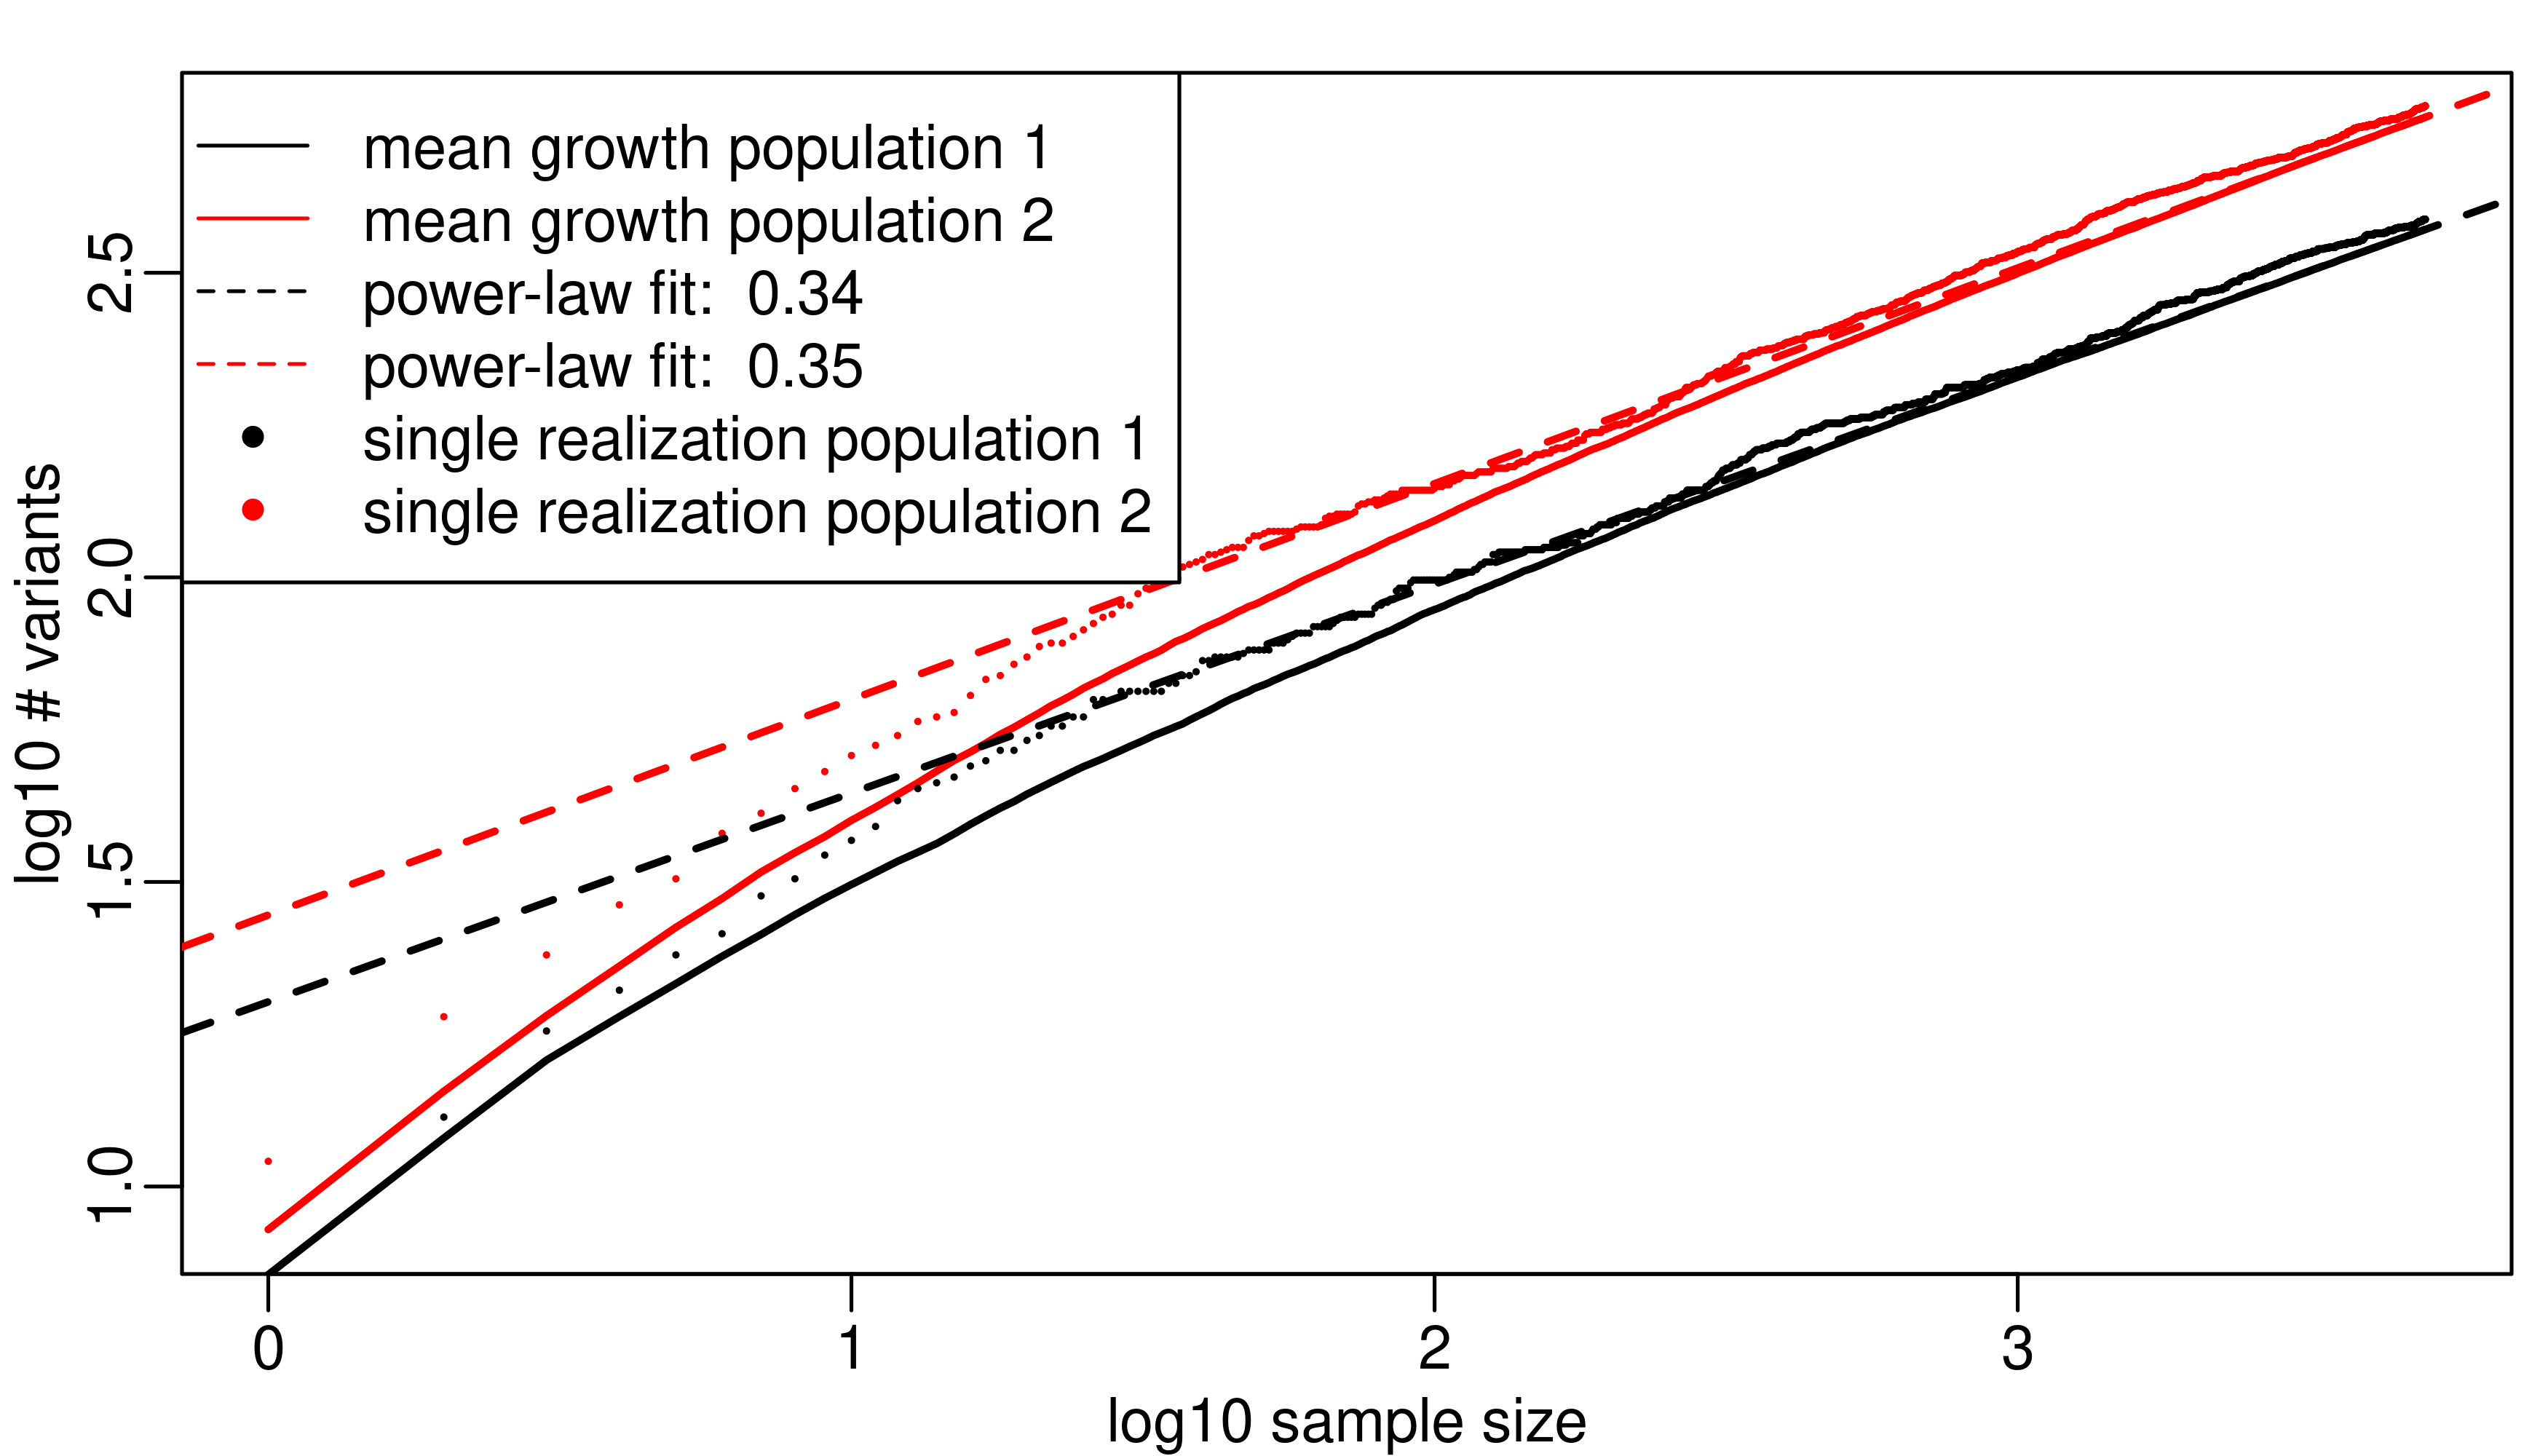
\includegraphics[width = 0.6\textwidth]{Ch2-double-trouble/Figs//powerlaw_simu_.3_.6_.5.png}
    \caption{Simulated sampling curve with $\mass = 10, \rate{1}=0.3, \rate{2}=0.6, \conc{1}=\conc{2}=1, \corr{i}=\corr{2}=0.5$ in the projection scheme, i.e. sampling population 1 or population 2 only. The mean growth curves (shown in lines) were calculated using 100 independent realizations and a single realization is shown as dots. The bound for population 2 is 0.3 and 0.6 and the predicted power law rate for population 1 is 0.3. We fit the line using the last 1/3 of the mean growth curve. The fitted powerlaw align well with our theoretical prediction.}
\end{figure}
